\section{Spazio}

Come citato poc'anzi quando si parla di suono bisogna considerare quindi lo spazio e il mezzo in cui l'onda si propaga.
Possiamo classificare gli spazi in diverse categorie, le principali sono (Davis - Pag 178):
\begin{itemize}
\item Free Field:
È definito così uno spazio uniforme, libero da ostacoli che potrebbero produrre delle riflessioni o rifrazioni e non contaminato da sorgenti sonore estranee.
Esempi di questo tipo sono le sale anecoiche (senza eco),camere particolari il cui scopo è quello di ridurre al minimo le riflessioni delle onde, utili per eseguire test precisi su apparecchiature audio.
\item Reverberant field:
È uno spazio chiuso, con pochissimo assorbimento acustico, in cui la pressione sonora è uniforme in ogni punto e le onde si propagano allo stesso modo in tutte le direzioni.
Caratteristiche di questo tipo possiamo trovarle in luoghi come camere vuote o cavità.
\item Semireverberant Field:
È il tipo di spazio più comune che possiamo incontrare, nel quale l’energia è sia assorbita che riflessa. L’energia si muove in più direzioni ma è comunque percepibile il punto di origine della fonte di generazione dell’evento sonoro.
\end{itemize}

\subsection{Risposta all'impulso}

Al giorno d’oggi conosciamo una tecnica in grado di eseguire una fotografia delle caratteristiche acustiche in grado di descrivere come il suono si propaga da un punto di emissione ad un ricevitore.

Parliamo di \textit{Risposta all’impulso} ovvero del modello fisico-matematico di un sistema lineare, non dipendente dal tempo, composto solo da un input ed un output\footcite{af:book}.

Le informazioni contenute sono sia relative al dominio del tempo, ad esempio riflessioni e ritardi nella propagazione che, relative al dominio della frequenza, comportando quindi modifiche dal punto di vista spettrale.

Il sistema utilizzato viene detto \textit{Black box} che, come detto in precedenza è composto da un singolo input ed un singolo output. All’interno di questa black box gli elementi che concorrono all’acquisizione dei dati matematici dello spazio che si vuole registrare sono:
\begin{itemize}
\item Un generatore di segnale: Tipicamente un pc;
\item Un amplificatore di segnale;
\item Un diffusore di segnale: il quale riproduce il segnale nello spazio in modo omnidirezionale;
\item Un ricevitore: un microfono anch’esso omnidirezionale, in quanto vogliamo escludere la direzionalità dallo studio.
\end{itemize}
Per misurare quindi la risposta all'impulso riproduciamo il segnale attraverso l’altoparlante nello spazio e contemporaneamente registriamo come, quel segnale, si propaga in quel determinato spazio e in quelle determinate condizioni, attraverso il microfono.

Il segnale originale consiste in uno sweep esponenziale il quale parte dalla frequenza $f_1$, termina a frequenza $f_2$ in $t$ secondi.

Il segnale riverberato conterrà al suo interno componenti spettrale non presenti nell’originale, che corrispondono alla risposta lineare in frequenza dello spazio.
Attraverso un processo di convoluzione, ampiamente spiegato e perfezionato dal prof. A Farina, siamo in grado di restituire la risposta all'impulso del sistema lineare.

È da tenere conto che però una singola registrazione non è in grado di descrivere tutto lo spazio. La risposta all’impulso, come già detto, è relativa soltanto al punto in cui è posizionato il ricevitore e soltanto per il punto da cui è emesso il suono. Per la mappatura dello spazio per restituire un'immagine fedele dello spazio sono necessarie numerose registrazioni. Come per una fotografia, maggiore è il numero di “pixel”, più definita sarà l’immagine. Per questo è un lavoro che, soprattutto per luoghi ampi, richiede moltissimo tempo e spesso si tende ad effettuare un numero di registrazioni non necessario a restituire un modello fedele.

\subsection{Storia dello studio degli spazi}

Storicamente, in ambito musicale, lo spazio è stato sempre presente ed essenziale durante le performance. Basti pensare agli auditorium greci, dove la conformazione permette sia un rinforzo in termini di ampiezza, ma anche una forte intelligibilità delle parole in modo tale da raggiungere chiaramente tutti i presenti.
Gli ascoltatori, posti ad un'angolazione di circa 120 gradi, ricevevano il suono diretto dall’oratore, seguito delle riflessioni provenienti sia dal pavimento dell’orchestra, che dal retro del palco, anche se con minor intensità.

\begin{figure}[h]
\centering
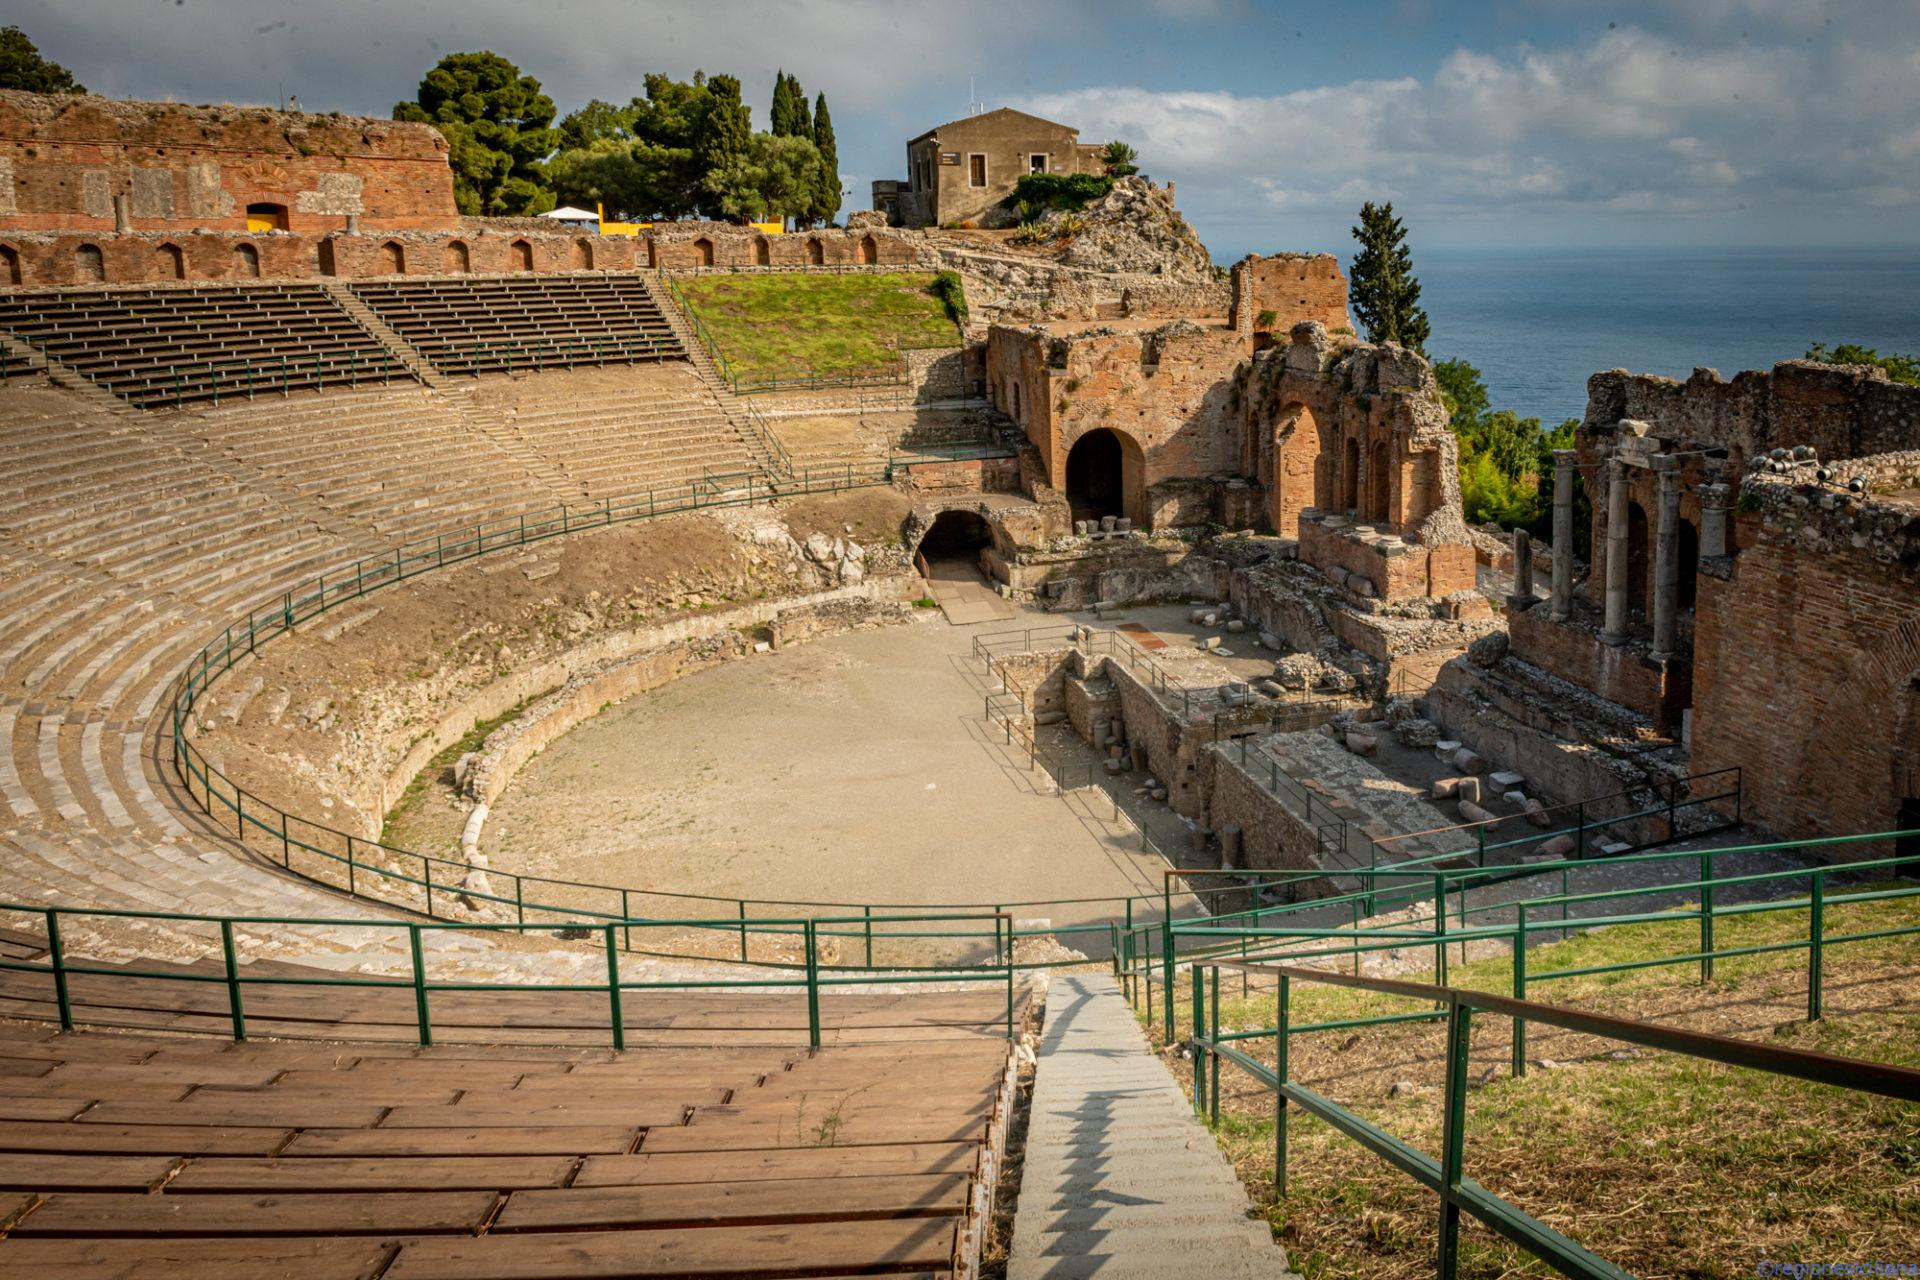
\includegraphics[width=%
0.50\textwidth]{teatrogreco}
\caption{Foto del teatro greco di Siracusa}
\label{fig:teatrogreco}
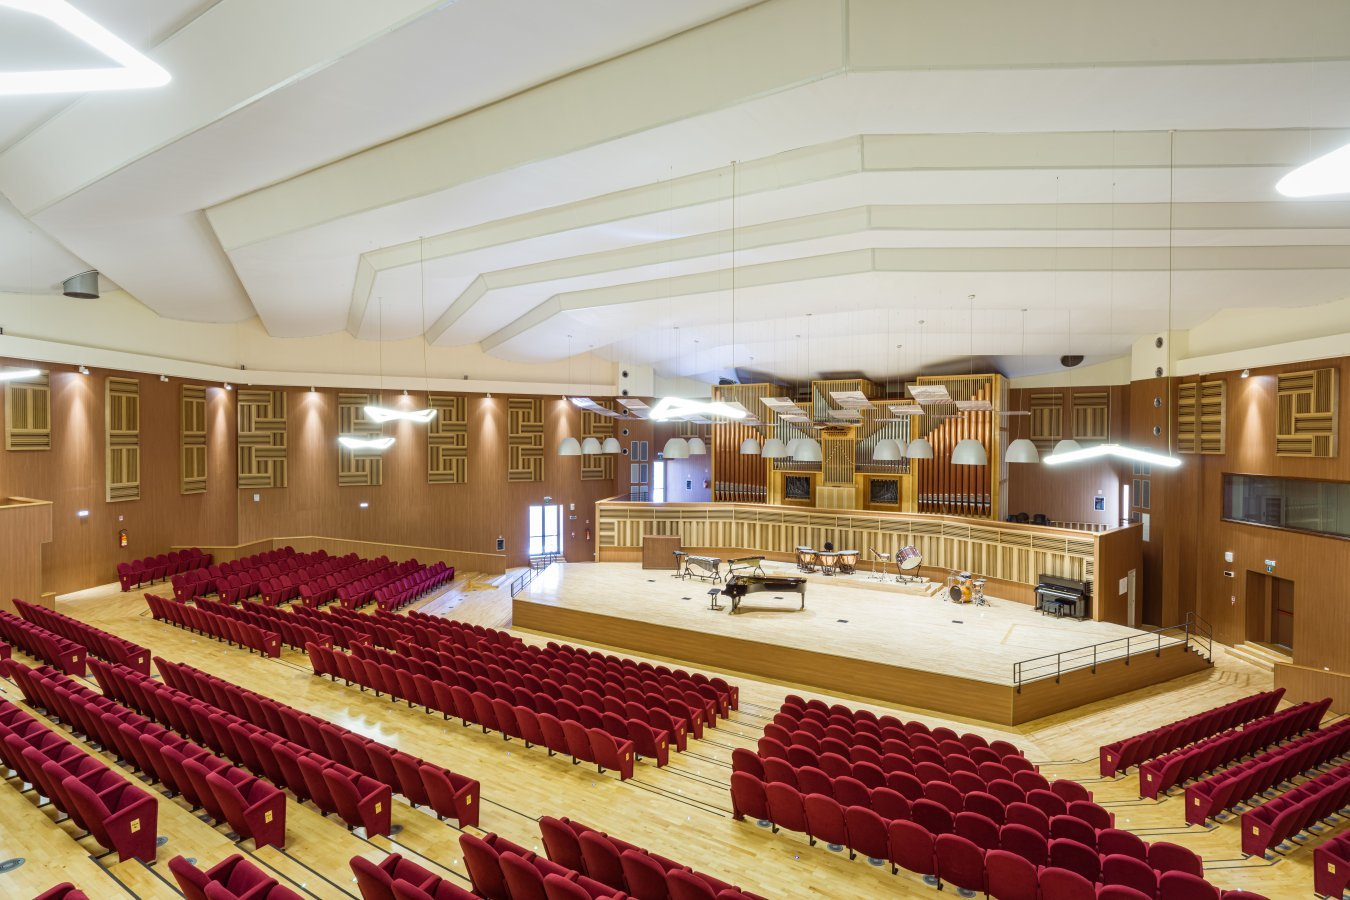
\includegraphics[width=%
0.50\textwidth]{auditorium}
\caption{Foto dell'auditorium Nino Rota del conservatorio di Bari}
\label{fig:auditorium}
\end{figure}

Il palco, inoltre, aveva un’ altezza compresa tra 1m e 3.6m, comportando una differenza nell’angolo di incidenza del suono diretto (Auditorium Acoustics and Architectural Design Di Michael Barron).
Infine, un altro accorgimento degli architetti greci, i quali avevano scoperto le proprietà di assorbimento, era il posizionamento tra le sedute di vasi contenenti ceneri, i quali avevano lo scopo di assorbire l’energia sonora che sarebbe stata riflessa indietro verso il palco.

Un’altro esempio in cui vediamo lo spazio come protagonista, è il caso degli organi, in cui il luogo è la vera e propria cassa armonica dello strumento.
L’acustica dell’organo è fortemente legata alla sua ubicazione, infatti, a differenza di altri strumenti musicali i quali possono essere spostati e trasportati, per l’organo non è possibile. Inoltre i luoghi provvisti di organo sono spesso molto riverberanti, come ad esempio le chiese e i teatri, e questo concorre alla definizione timbrica dello strumento

\begin{figure}[h]
\centering
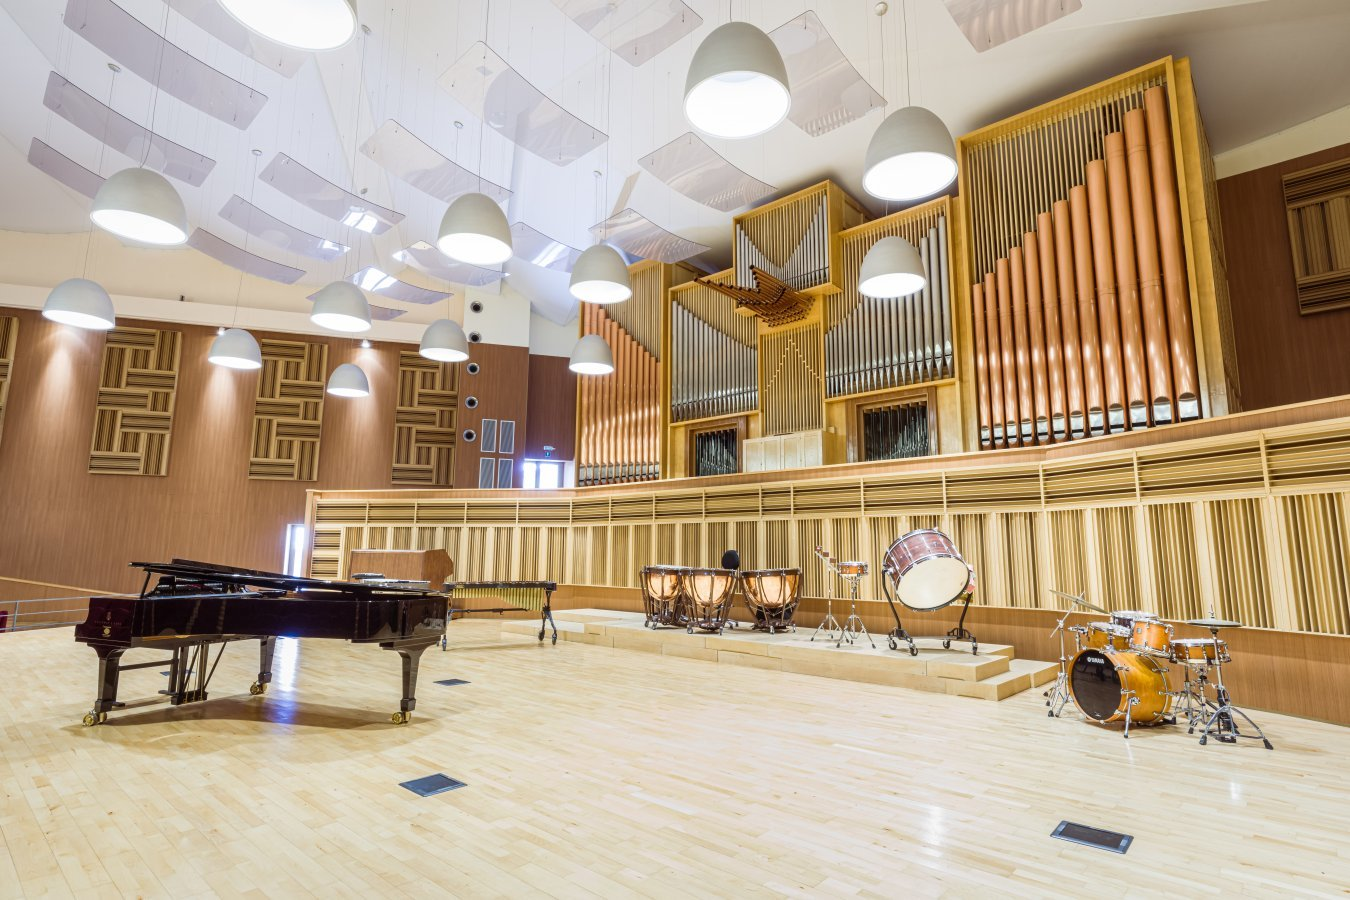
\includegraphics[width=0.80\textwidth]{organo}
\caption{Foto dell'organo presente nell'auditorium N.Rota}
\label{fig:organo}
\end{figure}

\subsection{Lo spazio come parametro}
Si è dovuto attendere però circa gli anni 60 affinchè lo spazio diventasse un vero e proprio parametro compositivo.

\emph{“Gesang der Jünglinge"} di Karlheinz Stockhausen è un’opera importantissima per l’epoca in cui è stata composta. Il brano, nato pentafonico e successivamente ridimensionato in quadrifonia, rappresenta l’avanguardia del serialismo integrale. Come accennato in precedenza, questo lavoro è il primo esempio in cui vediamo la gestione dello spazio come parametro compositivo, al pari di ampiezza, altezza e timbro.
Gli altoparlanti, disposti circolarmente attorno agli ascoltatori, creano uno spazio in cui immergersi permettendo complessi movimenti tra gli stessi.
Vengono infine introdotti termini quali “Intervallo spaziale” e “Accordi di spazio”.
